%%
%%  Department of Electrical, Electronic and Computer Engineering.
%%  EPR400/2 Final Report - Section 4.
%%  Copyright (C) 2011-2018 University of Pretoria.
%%

\section{Results}

\subsection{Summary of results achieved}

\begin{center}
	\begin{longtable}{|p{5cm}|p{5cm}|p{5cm}|}
		\hline
		\textbf{Description of requirement or specification (intended outcome)} &
		\textbf{Actual outcome} &
		\textbf{Location in report} \\
		\hline 
		\multicolumn{3}{|l|} {\textbf{Mission requirements of the product}} \\
		\hline
		Text recognition should
		consider the probability of
		occurance of combinations of
		letters.
		&
		The Viterbi algorithm was successfully implemented to detect the closest words which were in the user's dictionary.
		&
		Section 4.2.1
		\\
		\hline
		The user should be able to undo an input onto the touchscreen and not have the written sentence converted to text.
		&
		The device's GUI had a "Clear" button which had the capability of resetting the touchscreen to being blank when clicked.
		&
		Section 4.2.3\\
		\hline
		The system should recognize
		that the user has completed
		writing their shopping list.
		& 
		The device's software system correctly realized when user input was finished by keeping track of the "Finished" button on the GUI, which when switched the booolean variable that tracked if input was finished.
		&  Section 4.2.3\\
		\hline
		\multicolumn{3}{|l|} {\textbf{Field Conditions}} \\
		\hline
		The device should read handwriting input from multiple users.
		&
		The device could accurately recognize handwritings from multiple users. 
		&
		Section 4.2.8
		\\
		\hline
		The device should operate under varying light conditions that will be typical of what the user will encounter in indoor environments.
		&
		Operation of the device was executed in a dark room and in the presence of a bright fluorescent light. The device successfully carried out all its function in the two different light conditions.
		&
		Section 4.2.11
		\\
		\hline
		\multicolumn{3}{|l|} {\textbf{Specifications}} \\
		\hline
		Information should be sent at
		request, to the mobile phone
		within 10 seconds.
		&
		The measured time for the transmission time of the email containing the shopping list was found to have a mean of 8.35 s
		&   
		Section 4.2.2
		\\
		\hline
		Accuracy of the handwriting
		character detection must be
		greater than 80$\%$.
		&
		The average accuracy calculated from different unseen handwritings was found to be 83.3$\%$.
		&   Section 4.2.1\\
		\hline
		The user must be warned
		when the battery power
		remaining is less than 10$\%$ of
		full capacity.
		&
		An algorithm was programmed to continuously check the battery progress bar as a global variable of the project and when it reached less than $10\%$, a boolean flag for low battery was triggered.
		&	Section 4.2.9\\
		\hline
		Handwritten input must be converted to text by the character recognition software in less than 1s.
		&
		The average conversion time for a line sentence input was measured to be 690 m s, using the timer. 
		&
		Section 4.2.3\\
		\hline
		The communication link
		between the device’s
		communication system
		and the phone system should
		transfer data bidirectionally,
		at a rate of between 5Mbps
		and 10Mbps so that the bit
		error rate can be less than
		10$\%$.
		&
		The Wi-Fi link on the device could communicate at speeds of 11 Mbps.
		&
		Section 4.2.2
		\\
		\hline
		\multicolumn{3}{|l|} {\textbf{Deliverables}} \\
		\hline
		Optical character recognition algorithm for handwritten input to text conversion. The algorithm will be implemented on the hand-held shopping list device.
		&
		The optical recognition algorithm was successfully designed for and implemented onto the software system.
		&
		Section 4.2.1
		\\
		\hline
		Integration of the embedded processor
		board, the communication system and the touchscreen LCD to make the shopping list hardware device.
		&
		The different hardware was integrated to create the full working physical system which could be attached to a fridge.
		&
		Section 4.2.6 \\
		\hline	
		\caption{Results summary}
	\end{longtable}

\end{center}

\subsection{Qualification tests}

\subsubsection{Qualification test 1: Measurement of handwriting recognition accuracy}

4.2.1.a Qualification test\\
\textit{Objectives of test / experiment}\\
The accuracy of the handwriting scheme was measured in the test. The converted output was also checked against the dictionary and the relevant output was shown.

\textit{Equipment used}\\
The Python programming language was used. The mathematical libraries contained as well as the tracking libraries were used to develop an algorithm that could keep track of the recognized outputs and compare them to the expected values. The pseudo-code for the Python program implemented to calculate the accuracy of the recognition algorithm is shown below:\\

\begin{algorithmic}
	\STATE expectedOuputs.txt $\Leftarrow$ $\hfill$ $\rightarrow$ Text file containing expected text outputs.
	\WHILE {userInput == \textbf{true}}  
	\STATE \textbf{getUserLineInput()}  \hfill $\rightarrow$ Capture the user's handwritten shopping list line.
	\STATE sentence $\leftarrow$ \textbf{convertLineInput()} \hfill $\rightarrow$ Save recognition output
	\STATE dictionaryOut $\leftarrow$ Viterbi(sentence) \hfill $\rightarrow$ Detect closest word in dictionary.
	\STATE shoppingList.txt $\leftarrow$ dictionaryOutput \hfill Append the shopping list with the recognized sentence.
	\ENDWHILE
	\STATE correct = 0 \hfill $\rightarrow$ Correctly recognized letters
	\STATE total = 0 \hfill $\rightarrow$ Total recognized letters.
	\FOR {every line in shoppingList.txt}
	\FOR {every character i in every line}
	\IF {shoppingList.i == expectOutputs.i}
	\STATE correct $\leftarrow$ correct++ \hfill Increment correct characters
	\ENDIF
	
	total $\leftarrow$ total$++$ \hfill Increment total detected characters
	\ENDFOR
	\ENDFOR
	
	\STATE accuracy  $=$ $\frac{\text{correct}}{\text{total}} \times 100\%$
\end{algorithmic}

\textit{Experimental Parameters and setup}\\
The above values of accuracy were the important test parameters and the algorithm was implemented in Python.

\textit{Experimental protocol}\\
The basic steps in the calculation of the accuracy were extracted from the comments in the pseudo-code above:
\begin{itemize}
	\item Take the user input and convert to the corresponding sentence.
	\item Take the sentence and convert its contents to relevant dictionary words.
	\item Compare every letter from this output to the expect shopping list contents.
	\item Calculate output value.
\end{itemize}

4.2.1.b Results and Observations\\\\
\textit{Measurements}
\begin{center}
	\begin{longtable}{|p{5cm}|p{5cm}|}
		\hline
		\textbf{Number of sentences} &
		\textbf{Average Accuracy ($\%$)} \\
		\hline
		5
		&
		92.5
		\\
		\hline
		10
		&
		88.76
		\\
		\hline
		15
		&
		81.95
		\\
		\hline
		20
		&
		78.32
		\\
		\hline
		30
		&
		82.81
		\\
		\hline
		\textbf{Cumulative accuracy}
		&
		84.87
		\\
		\hline		
		\caption{Accuracy results}
	\end{longtable}
\end{center}

\begin{figure}[h]
	\centering
	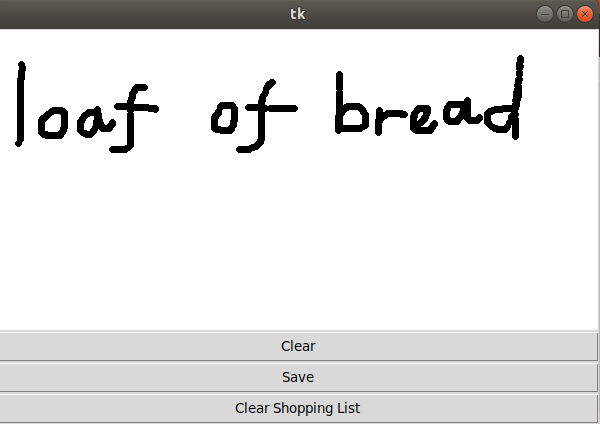
\includegraphics[scale=0.4]{101}
	\caption{First line user input}
\end{figure}

\begin{figure}[h]
	\centering
	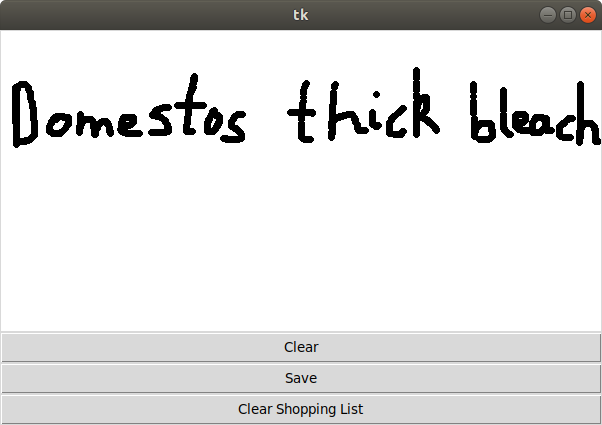
\includegraphics[scale=0.4]{102}
	\caption{Second line user input}
\end{figure}

\begin{figure}[h]
	\centering
	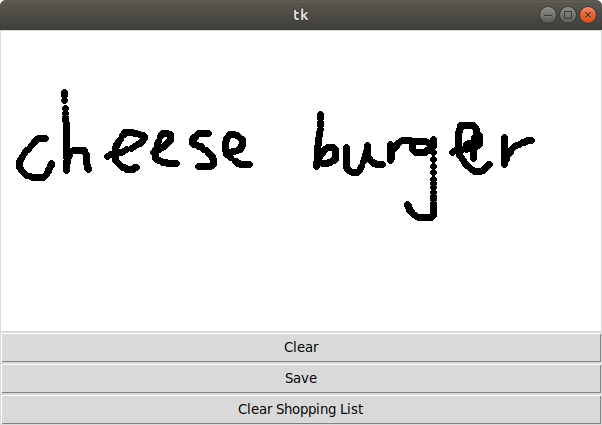
\includegraphics[scale=0.4]{103}
	\caption{Third line user input}
\end{figure}

\begin{figure}[h]
	\centering
	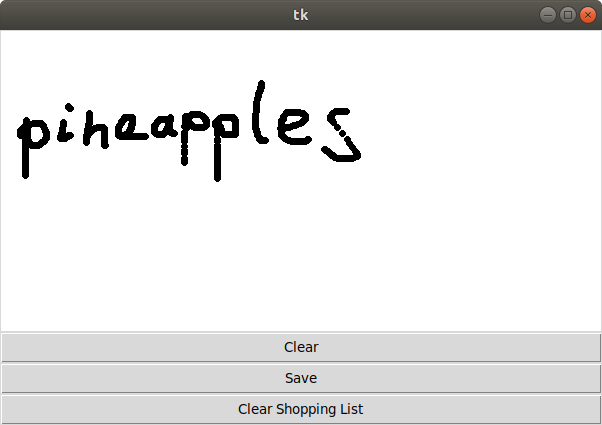
\includegraphics[scale=0.4]{105}
	\caption{Fifth line user input}
\end{figure}

\begin{figure}[h]
	\centering
	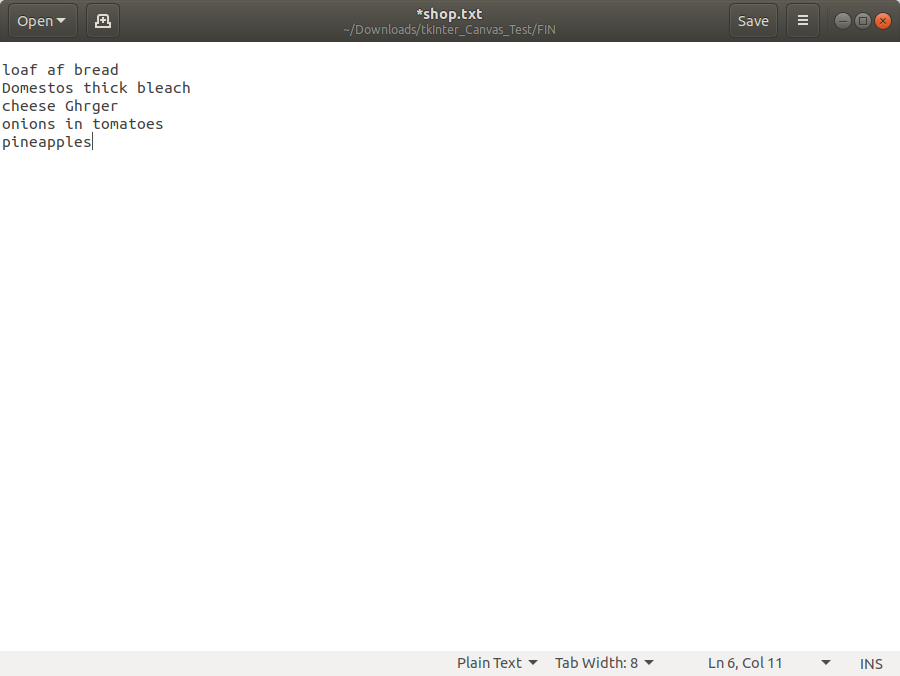
\includegraphics[scale=0.4]{106}
	\caption{Output text file containing shopping list}
\end{figure}
\clearpage
\textit{Description of results}\\
The accuracy of the recognition algorithm decreased as the number of sentences were doubled from 5 to 10. The accuracy decreased again as 5 more lines of user input were inserted. Addition of another 5 lines decreased the accuracy. Adding 10 more lines of user input led to an increase in the accuracy. The general accuracy was calculated to be 84.87$\%$

\subsubsection{Qualification test 2: Measurement of the transmission time for sending email}

4.2.2.a Qualification test\\
\textit{Objectives of test / experiment}\\
The time taken to send an email from the shopping list device to the user's email address. The wireless network's link capacity was also checked. 

\textit{Equipment used}\\
A Quartz stopwatch was used for timing.
\\

\textit{Experimental parameters and setup}\\
The value of $t_{transm}$ was the transmission time of note between the shopping list device sending the email and the message appearing on the user's inbox. The assumption was that the user had their e-mail service auto-refreshing at period of less than a second so that a new message was recognized immediately.

\textit{Experimental protocol}\\
The stages that were involved with the experiment were:
\begin{itemize}
	\item Reset the stopwatch to zero and open the email service on the user's phone.
	\item Run the mail algorithm code and simultaneously press the start button.
	\item Wait for the new email notification to pop up on the user's phone.
	\item  Stop the stopwatch when the email notification is observed by the user.
\end{itemize}

4.2.2.b Results and Observations\\
\textit{Measurements}\\
\begin{center}
	\begin{longtable}{|p{5cm}|p{5cm}|}
		\hline
		\textbf{File size (kiloBytes)} &
		\textbf{Transmission time (s)} \\
		\hline
		0.5
		&
		1.22
		\\
		\hline
		0.78
		&
		1.48
		\\
		\hline
		1.2
		&
		2.24
		\\
		\hline
		5.65
		&
		3.32
		\\
		\hline
		500
		&
		7.95
		\\
		\hline		
		\caption{Transmission time values.}
	\end{longtable}
\end{center}

\textit{Description of Results}\\
The first test was implemented for a file with 10 different sizes and of size 500 Bytes. The transmission time was extremely small. A few more lines were added and the transmission time was fast as well, only slower by a few hundredths of seconds. The lines of the text file were almost doubled and the transmission time increased by about a second. A bigger file i.e. an image was sent as the next argument and the transmission time was slower than the previous one by a second. A \textbf{.pdf} file was the file document sent by the e-mail system and although it was about 100 times larger than the previous file sent, it was only delivered in double the transmission time of the smaller file.

\subsubsection{Qualification test 3: System detection of user finishing handwriting process and handwriting conversion}

4.2.3.a Qualification test\\
\textit{Objectives of text / experiment}\\
The test involved the detection of the end of a user input process for their line sentence and the conversion of the line input in less than 1 second.

\textit{Equipment used}\\
The internal timing libraries of the Python environment were used. The Widget libraries were used to create GUI buttons which were kept track of by boolean variables. The pseudo-code for the conversion time calculation was shown below:\\

\begin{algorithmic}
	\STATE saveButton.clicked $\leftarrow$ \textbf{false} \hfill Initialize an unclicked button for save functionality  
	\WHILE {saveButton.clicked==\textbf{false}}
	\STATE drawn $\leftarrow$\textbf{false} userDrawing \hfill Model the input drawn
	\ENDWHILE
	\STATE $\rightarrow$ saveButton has now been clicked
	\STATE \textbf{startTimer()}
	\STATE convertInput \hfill $\rightarrow$ Apply Recognition algorithm
	\STATE \textbf{stopTimer()}
	\STATE $t_{reco}$ $\leftarrow$ timerValue	\hfill Recognition time value
\end{algorithmic}

\textit{Experimental Protocol}\\
The flow chart in Figure 36 shows the stages of the experimental protocol. 
\newpage
\begin{figure}[h]
	\centering
	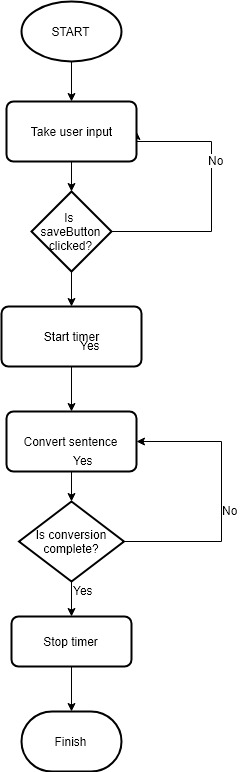
\includegraphics[scale=0.5]{50}
	\caption{Flow chart showing the experiment protocol}
\end{figure}

4.2.3.b Results and Observations\\
\textit{Measurements}\\
\begin{center}
	\begin{longtable}{|p{5cm}|p{5cm}|}
		\hline
		\textbf{Sentence number} &
		\textbf{Conversion time (s) ($\%$)} \\
		\hline
		1
		&
		0.43
		\\
		\hline
		2
		&
		0.88
		\\
		\hline
		3
		&
		0.32
		\\
		\hline
		4
		&
		0.65
		\\
		\hline
		5
		&
		0.49
		\\
		\hline
		\textbf{Average Conversion Time}
		&
		
		\\
		\hline		
		\caption{Accuracy results}
	\end{longtable}
\end{center}

\textit{Description of Results}\\

\newpage

%% End of File.


